%%%%%%%% ICML 2024 EXAMPLE LATEX SUBMISSION FILE %%%%%%%%%%%%%%%%%

\documentclass{article}

% Recommended, but optional, packages for figures and better typesetting:
\usepackage{microtype}
\usepackage{graphicx}
\usepackage{subfigure}
\usepackage{booktabs} % for professional tables

% hyperref makes hyperlinks in the resulting PDF.
% If your build breaks (sometimes temporarily if a hyperlink spans a page)
% please comment out the following usepackage line and replace
% \usepackage{icml2024} with \usepackage[nohyperref]{icml2024} above.
\usepackage{hyperref}


% Attempt to make hyperref and algorithmic work together better:
\newcommand{\theHalgorithm}{\arabic{algorithm}}

% Use the following line for the initial blind version submitted for review:
% \usepackage{icml2024}

% If accepted, instead use the following line for the camera-ready submission:
\usepackage[accepted]{icml2024}

% For theorems and such
\usepackage{amsmath}
\usepackage{amssymb}
\usepackage{mathtools}
\usepackage{amsthm}

% if you use cleveref..
\usepackage[capitalize,noabbrev]{cleveref}

%%%%%%%%%%%%%%%%%%%%%%%%%%%%%%%%
% THEOREMS
%%%%%%%%%%%%%%%%%%%%%%%%%%%%%%%%
\theoremstyle{plain}
\newtheorem{theorem}{Theorem}[section]
\newtheorem{proposition}[theorem]{Proposition}
\newtheorem{lemma}[theorem]{Lemma}
\newtheorem{corollary}[theorem]{Corollary}
\theoremstyle{definition}
\newtheorem{definition}[theorem]{Definition}
\newtheorem{assumption}[theorem]{Assumption}
\theoremstyle{remark}
\newtheorem{remark}[theorem]{Remark}

% Todonotes is useful during development; simply uncomment the next line
%    and comment out the line below the next line to turn off comments
%\usepackage[disable,textsize=tiny]{todonotes}
\usepackage[textsize=tiny]{todonotes}


% The \icmltitle you define below is probably too long as a header.
% Therefore, a short form for the running title is supplied here:
\icmltitlerunning{Predictive Coding Networks and Free Energy}

\begin{document}

\twocolumn[
\icmltitle{Understanding the Robustness and Generalizability of 
            Predictive Coding Networks and Free Energy}

% It is OKAY to include author information, even for blind
% submissions: the style file will automatically remove it for you
% unless you've provided the [accepted] option to the icml2024
% package.

% List of affiliations: The first argument should be a (short)
% identifier you will use later to specify author affiliations
% Academic affiliations should list Department, University, City, Region, Country
% Industry affiliations should list Company, City, Region, Country

% You can specify symbols, otherwise they are numbered in order.
% Ideally, you should not use this facility. Affiliations will be numbered
% in order of appearance and this is the preferred way.
\icmlsetsymbol{equal}{*}

\begin{icmlauthorlist}
\icmlauthor{Rohit Mohnani}{brown}

\end{icmlauthorlist}

\icmlaffiliation{brown}{Brown University}


% You may provide any keywords that you
% find helpful for describing your paper; these are used to populate
% the "keywords" metadata in the PDF but will not be shown in the document
\icmlkeywords{Machine Learning, ICML}

\vskip 0.3in
]

% this must go after the closing bracket ] following \twocolumn[ ...

% This command actually creates the footnote in the first column
% listing the affiliations and the copyright notice.
% The command takes one argument, which is text to display at the start of the footnote.
% The \icmlEqualContribution command is standard text for equal contribution.
% Remove it (just {}) if you do not need this facility.

%\printAffiliationsAndNotice{}  % leave blank if no need to mention equal contribution
% \printAffiliationsAndNotice{\icmlEqualContribution} % otherwise use the standard text.

\begin{abstract}
Inference Learning (IL) and their use in Predictive Coding Networks (PCNs)
provide a biologically plausible alternative to the standard Backpropagation
algorithms used in conventional Artifical Neural Networks (ANNs). Recent work
has been done to make IL more computationally competitive and thus viable for use 
in large scale models.\cite{alonso2024understanding} In this paper, we test these 
proposed computationally efficient and performant models on more challenging Image
Classification datasets in order to further investigate its capabilities and limitations. 
\end{abstract}

\section{Introduction}

Backpropagation (BP) is the go-to algorithm for gradient estimation 
used to train neural networks because it is unreasonably effective.
It is computationally efficient, it often seems to work well 
\cite{LeCuBottOrrMull9812}, and is able to take advantage of modern 
GPU-based computing to further parallelize its computations thus 
reducing training times. However, there are various features of 
BP that make it irreconcilable with neurobiological processes. The main
three are as follows:

\begin{itemize}
    \item \textbf{Symmetric weights}: Neurons fire electrical signals in one
            direction, thus having weights be copied across both 
            feedforward and feedback signals is unrealistic
    \item \textbf{Exact Gradients}: BP requires precise gradient calculation
            using the chain rule, however in-brain processes are more probabilistic.
    \item \textbf{Global Information}: BP relies on a global error signal
            being propagated backwards to evaluate overall network performance.
            Biological systems don't have a global loss function to govern learning,
            hence the generalizability to learning various tasks. They instead rely 
            on local information to make changes at individual synapses to learn.
\end{itemize}

We have always looked to nature for inspiration because there are various things
that evolution has done very well that we can yet learn from. One famous
example is the Bullet train redesign in Japan. Bullet trains used to make
sonic booms when travelling through tunnels, and to solve this problem 
engineers redesigned the head of the train to mimic the shape of Kingfisher's
beak. This served to make it quieter, experience less air resistance and thus faster.

The case for PCNs is much the same. BP works very well, but perhaps there are 
still improvements to be had from more closely mimicing brain-based learning. 
PCNs are based on the idea that the Brain effectively maintains a model of 
the world and is constantly trying to predict sensory input and updates its model
by minimizing the discrepancy between predicted and observed signals. 

Most BP alternatives either fail to completely get over the biological
implausibility issues BP itself deals with or, if they do, perform signifcantly
worse than BP. PCNs are a promising alternative, made especially more so 
with the recent advancements made by Alonso et al. 

PCNs are implemented as Recurrent Neural Networks (RNNs) trained with Inference Learning (IL).
Their recurrent connections makes it so that feedforward and feedback connections 
interact with each other and are not segregated like in BP. IL has two phases:
Inference and Weight Update. In the Inference Phase, it generates predictions 
about sensory input and compares them with observations; this minimizes 
prediction errors, also known as free energy, with respect to neuron activities.
In the next phase IL implements hebbian-like localized updates to the network's 
weights to further minimize free energy. 

IL has suffered to gain traction primarily because it is significantly more
computationally expensive than BP, while the benefits it offered for that 
price were merely comparable performance at best. However, recent 
developments claim to solve most, if not all, of those issues through 
adjustments to the algorithm and the use of novel optimizers \cite{alonso2024understanding}.

In this paper, we set out to test their optimization techniques and model 
architectures on more diverse and challenging image classification datasets.
These techniques were initially tested on CIFAR-10 and MNIST, which are both
small datasets with only 10 output classes. We will test them on CIFAR-100, 
LabelMe50k, and Caltech-256.

In sum, while some of our results back claims made by the paper by Alonso et al 
which we base this paper on, there are also results that suggest some limitations 
that first need to be tackled, and that much more testing is required of these 
novel methods before we can definitively put PCNs and IL on par with BP.


\section{Background}

In a traditional neural network the error is something that expresses
the difference between the output of the network and the target/actual 
output. This error exists only at the output node of the model and is 
what is used in BP to propagate a signal back through the network to 
determine gradients and adjust weights. In PCNs however, error is something
that exists at every layer and indeed at every node, this is how it localizes
gradient estimation and updates. 

\begin{figure}[ht]
% \vskip 0.2in
\begin{center}
\centerline{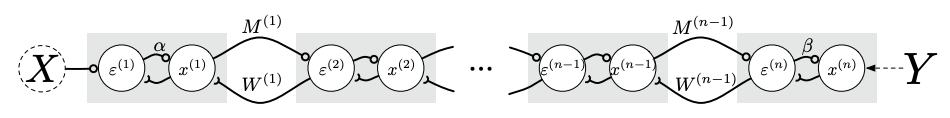
\includegraphics[width=\columnwidth]{images/pc_arch.png}}
\caption{Example PCN architecture}
\end{center}
% \vskip -0.2in
\end{figure}

This model shows a compactified view, where each node represents a layer
of nodes. \( x^{(i)}\) is a state node in the i-th layer, \( \epsilon^{(i)}\) is 
the corresponding error node in the i-th layer, while \(M^{(i)}\) and \(W^{(i)}\)
are the forward and backward weight matrices following the i-th layer. \(\alpha\) and \(\beta\)
are terms that are set to either 0 or 1 to clamp either end of the network. Different combinations 
of these values configure the model for different tasks. For training, we 
set \(\beta = 0, \alpha = 1\) to ensure output layer doesn't change but that 
the input exerts influence on the input layer. For discriminating, we set \(\beta = 1, \alpha = 1\)
allowing information to flow up the network and alter the output layer, once equilibirium 
is achieve the resultant value is the output of the model. There is even work 
being done on using \(\beta = 0, \alpha = 0\) to allow the input layer to change independently 
of the input to use it as a generative model in the vein of increasingly popular generative AI model 
\cite{orchard2019making}.

\begin{align}
    \tau \frac{d\varepsilon^{(i)}}{dt} &= x^{(i)} - M^{(i-1)}\sigma(x^{(i-1)}) - \nu^{(i)}\varepsilon^{(i)} \label{eq:1} \\
    \tau \frac{dx^{(i)}}{dt} &= W^{(i)}\varepsilon^{(i+1)} - \sigma_0(x^{(i)}) - \varepsilon^{(i)} \label{eq:2}
\end{align}

These are the equations used to update the state and error nodes for each layer.
Here \(\tau\) is a time constant, \(\nu\) is a scalar variance parameter, and \(\sigma\) is an
activation function. These updates are performed during the inference phase, and once equilibrium is reached, from 
these equations we can show that \(\varepsilon^{(i)} = (x^{(i)} - \mu^{(i)}) / \nu^{(i)} \label{eq:3}
\).

\(\mu^{(i)}\) here is the prediction for the state node at the ith layer being sent from the 
layer below it. \(\mu^{(i)} = M^{(i-1)} \sigma(x^{(i-1)}) \label{eq:4}\).
We can thus see that \(\epsilon^{(i)}\) is simply a measure of the difference between the predicted
activity/state of the node and its actual state scaled by some constant \(\nu\).

The Free Energy Principle (FEP) is a concept in neuroscience that suggests 
the Brain reduces 'surprise' by making predictions of the external world 
based on internal models for it which are updated using sensory input. If we use 
the squared error cost function to measure the 'surprise' we find that:
\(F_i  = \frac{1}{2}\left\| x^{(i)} - \mu^{(i)}\right\|^2 
= \frac{\nu^{(i)}}{2}\left\| \epsilon^{(i)} \right\|^2 \).
Here \(F_i\) is the Free-energy for layer i in the model. Thus the total Free Energy
is given by: \( F = \sum_{i=1}^{n} F_i = \sum_{i}^{n} \frac{\nu^{(i)}}{2}\left\| \epsilon^{(i)} \right\|^2\). 
This 'surprise' which refers to the difference between predictions and observations is 
called free-energy, and thus the objective that we minimize in this model and is theorized to be minimized 
in our brains is simply the sume of the prediction errors \(\epsilon\).

In the Inference Phase, neuron activites are intialized to feedforward activities \(x\) and then 
are updated to minimize the free energy, \(F\). Activities are updated over many iterations using 
the partial gradients of local prediction errors, while local errors are updated using partial 
gradients of local activities. 

In the Weight Update Phase, the weights \(M, W\) are further updated to minimize \(F\). These updates
utilize local error gradients: 

\begin{align}
    \gamma \frac{dM^{(i-1)}}{dt} = -\epsilon^{(i)} \otimes \sigma{(x^{(i-1)})} \\
    \gamma \frac{dW^{(i-1)}}{dt} = -\sigma{(x^{(i-1)})} \otimes \epsilon^{(i)}
\end{align}

These are the theoretical foundations of PCNs and the IL algorithm they employ.
In the next part of the paper, I will talk about the various limitations Alonso et al
claim to have overcome through their optimization techniques.

\section{Review of Existing Work}

\subsection*{Existing Issues}

While the PCN model is biologically plausible, the main drawback that
hindered its mass adoption is that it is computationally expensive 
compared to BP algorithms and does not provide enough benefit to make 
that tradeoff worth making.

During the Inference phase, feedforward layer activities are updated iteratively
using partial gradients of local errors. These updates are typically performed 
for 15+ iterations. Thus, while the Inference Phase is a feature that is novel 
and introduced to better mimic the brain it imposes heavy computational requirements
of the IL algorithm and is where most of the computational cost comes from.

In addition to this IL algorithms often converge to poor minima without the use 
of parameter-wise adaptive learning rates such as those employed in the Adam optimizer.
However optimizers like Adam, which are also typically used with BP algorithms, are very 
memory intensive and drive up the computational cost. In the case of BP, which is computationally
efficient in determining gradients, Adam is often used as the optimizer because the tradeoff of more memory 
for faster and more optimal convergence is worth it. However, in the case of IL 
which itself is computationally demanding, the added cost of needing to use Adam for comparable 
perfomance is another point against its utility. Recent work done by Alonso et al has made major strides in attempting to tackle these 
main issues \cite{alonso2024understanding}. 

\subsection*{Inference Phase}

Updating feedforward activites for T iterations,
typically involves an associated \(T(2L-1)\) where L is the number of layers in the network. 
Prior to their work a minimum of \(T >= L - 2\) iterations were required in order to ensure
non-zero errors formed at each hidden layer of the network. And in general, larger networks 
employing more layers will require more iterations to appropriately propagate errors through them.
In the standard method, errors are computed at each layer and then these errors are used to update 
activities according to the equations aforementioned. In this method, activities are updated simultaneously
at each iteration. Since updates are only performed to incorporate information from neighbouring layers,
it is evident that while the last layer may require no more updates after the first iteration, after the first 
iteration the first layer has only incorporated information from the second layer. However, the second layer
is yet to incorporate information from the newly updated 3rd,4th,.. layers and so on and so forth.
In essence, there is a lag in information spread from farther layers, and the further two layers are 
from each other the greater the lag.

Alonso et al propose an alternative way to update activities which they term 
Sequential Inference. In this method, activties for each layer are computed 
one at a time starting from the last layer going back. This ensures that all 
when we calculate any given layer's activity we are doing so with the requisite
information. Previous computations for activites for later layers in the network are
thus inherently baked into the current calculation, meaning the activity requires no further 
computations and thus allowing each layer to achieve non-zero errors within a single iteration.

This change further meant, that they could now truncate the Inference phase iterations.
Where previously on the order of L iterations were required to achieve non-zero errors, 
with Sequential Inference, they were now able to do it in 1. Thus only a few iterations were needed 
to effectively reduce Free energy with respect to the neuron activities. They settled on \(T = 3\)
for their inference iterations, which is considerably smaller and thus much more computationally 
competitive compared to previous requirements of at least 15 and growing with larger models.

\begin{figure}[ht]
    % \vskip 0.2in
    \begin{center}
    \centerline{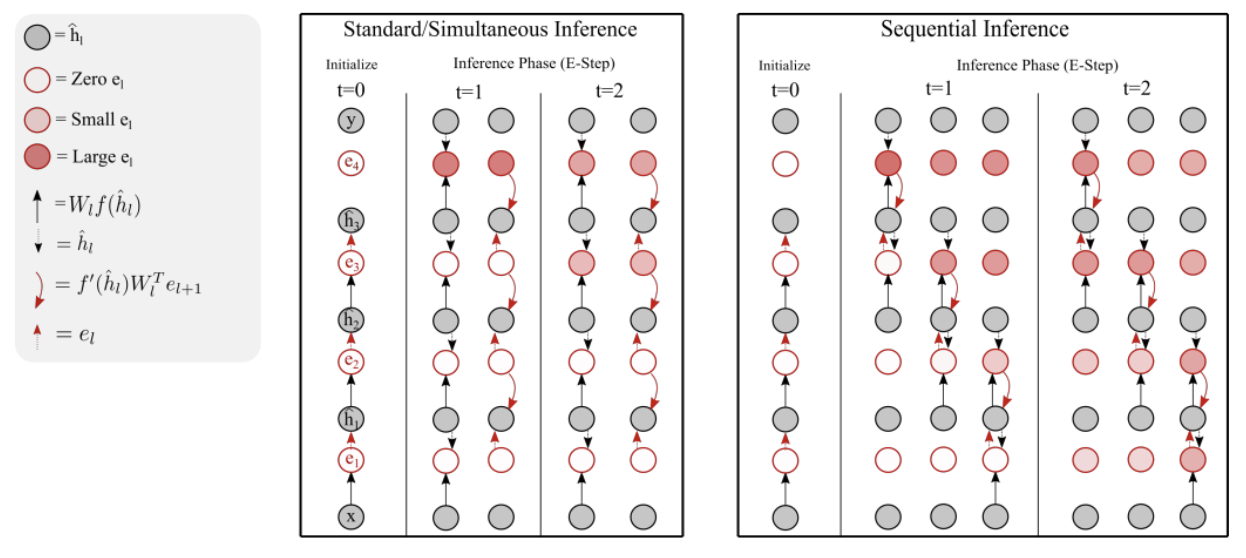
\includegraphics[width=\columnwidth]{images/seq_il.png}}
    \caption{Simulataneous Inference vs Sequential Inference}
    \end{center}
    % \vskip -0.2in
\end{figure}

\subsection*{Optimizer}

Alonse et al propose a novel optimizer called the Matrix Update Equalization
(MQ) Optimizer made specifically for the IL algorithm. IL often converged to poor
minima without the use of an optimizer like Adam, but Adam and other similar optimizers 
were too memmory intensive. They sought to make an optimizer that offered the same benefits
as Adam but without the significant computational overhead.

They based its design off of two key observations. One was that IL updates tend to 
be very, very small especially at early layers which offer a possible explanation as
to why it likely gets caught in local minima near its initialization values. Two was that
using matrix-wise scalar learning rates makes IL sensitive to second and higher order 
information. 

The MQ optimizer uses an adaptive single scalar learning rate per layer that prevents 
overly small update magnitudes and better equalizes these magnitudes between 
matrices. It employs a constant matrix-wise scalar learning rate \(\alpha_l\) for 
each matrix \(W_l\), as well as a global minimum learning rate \(\alpha_{min}\) and a 
matrix-wise scalar \(v_l\) which adapts to the moving average of the update magnitude.
Thus the weight update is given by this equation:

\begin{equation}
W_{l}^{(b+1)} = W_{l}^{(b)} - (\frac{\alpha_{l}}{v_{l} + r} + \alpha_{min}) \frac{\partial F}{\partial W_{l}^{(b)}}
\end{equation}

The moving average is updated every iteraion b, using row and column sizes \(i, j\), the L-1 norm 
of the gradient, and a global hyperparameter \(\rho\) with the followig equation:

\begin{equation}
v_{l}^{(b+1)} = (1 - \rho)v_{l}^{(b)} - \rho \frac{1}{ij} \left| \frac{\partial F}{\partial W_{l}^{(b)}} \right|
\end{equation}

They further claim that employing MQ puts IL on the same Order of Memory use, which they use model parameters and 
optimizer/algorithm parameters as a proxy for. Their research shows the MQ is able to reduce the differences in update magnitudes 
between the weight matrices comparably to Adam and prevents it from having small update magnitudes
at early layers. However, it is important to note that this result was obtained on the 
specific configuration of a Multi-Layer Perceptron (MLP) consisting of 3 hidden layers.


\subsection*{Limitations}

The datasets they used to test their optimizations on were small as were the model 
architectures they used. They primarily used the MNIST and CIFAR-10 datasets. MNIST is the 
handwritten digit recognition dataset consisting of 70,000 images where each image is 28 x 28 
in dimension. CIFAR-10 is a basic object recognition dataset consisting of 60,000 images of 
32 x 32 dimension. Both datasets have only 10 output classes. Both were tested on using 
a model with 3 convolutional layers and 1 linear layer. While this is the correct first step 
in testing out these novel ideas and techniques, much more testing is required to determine 
the robustness and generalizability of the ideas put forth in their paper. That is the goal 
of this paper: to further test their methods against more difficult datasets and see how far 
these advancements can take us.

\section{Datasets}

\subsection*{CIFAR-100}

CIFAR-100 is very similar to its CIFAR-10 counterpart. This dataset consists of 
60,000 images again of 32 x 32 dimension, but instead of having 10 output classes 
it features 100 output classes \cite{cifar100}. This dataset has 600 images per class and is split into
50,000 train images and 10,000 test images. It also has 20 superclasses which the 100 classes 
are grouped into, but for the purposes of our experiments this additional class was not used.

While the image dimension and quantity haven't changed in comparison to the image set
used by Alonso et al, a key difference here is the larger number of classes of 100 compared
to 10. This dataset is used to test whether these optimizations can provide comparable 
improvements even when used on more diverse datasets with larger classification spaces.

\subsection*{LabelMe\_12\_50k}

LabelMe\_12\_50k provides the first big departure from the image datasets used in the original 
paper. This dataset consists of 50,000 images split into 40,000 for training and 10,000
for testing \cite{labelme50k}. Each Image has dimension 256 x 256 which is significantly larger than the previous 
images used. 50\% of the images show a centred object, while the rest show a randomly selected region 
of a randomly selected 'clutter' image. It has 12 output classes and the distribution of images 
is maintained in each of the training and testing sets. 

This dataset is supposed to provide a challenge to object recognition algorithms 
because instances of each class vary wildly in appearance, lighting condition, and viewing angle.
Further centred objects may be partly occluded while other objects may be present in the image.
This dataset is used to test the model's robustness compared to BP. One advertized strength of 
PCNs is their robustness to noise which this dataset has a lot of, as well as to see how well it is 
able to perform for larger inputs and larger models.

\subsection*{Caltech-256}

Caltech-256 is the successor to Caltech-101. It features 30,607 images spanning 
257 object categories, which are themselves very diverse \cite{caltech256}. Each category 
has a minimum of 80 images, with the distirbution having a median of 100, mean of 117 and max of 
827. 

It is important to note that unlike the previous two datasets, this dataset's images do not have standardized dimensions. 
In the preprocessing for the data, I resized all images to a standard size of 256 x 256, which is the size 
of the input images for the LabelMe50k dataset.

\section{Experimental Setup}

The code written for the original paper \cite{alonso2024understanding} is publicly available at a 
github repository \href{https://github.com/nalonso2/PredictiveCoding-MQSeqIL/tree/main}{here}. My first steps 
involved familiarizing myself with their codebase as well as fixing issues such as missing files, computer 
architecture differences that made it so that it wasn't runnable out of the box. Once I was able to run their models 
without errors, my next step was to determine what parameters I would use for my own experiments. 

While the original paper used epochs on the order of 50 and 100 for their models, my hardware did not afford me the same 
computational capabilities. As I was running all these tests locally on my M2 Macbook Pro, even with GPU acceleration courtesy of 
pytorch's MPS backend which takes advantage of the Metal Programming framework on macbooks, my compute was severy limited. Even small models 
going till 15 epochs would take upwards of an hour to run. As for the other hyperparameters, I simply carried forwards the optimal 
hyperparameters described in the paper, as again the resources required to determine optimal hyperparameters were out of both 
my compute and time budget. 

While the CIFAR-100 and Caltech-256 datasets could be accessed through torchvision.datasets, the LabelMe50K 
dataset was not. I had to download the dataset locally and write a custom dataset class for it, making use of the annotations file
provided to iterate over all the images and match each with its label. In the data loading step I also had to apply 
transformations to the Caltech-256 dataset to make sure the images were resized to a standard dimension which I arbitrarily
chose to be 256 x 256. 

For the LabelMe50k datasets I used a small CNN model. This model had 3 convolutional layers with kernel size of \((7,7)\)
and stride of \((2,2)\). After each convolutional layer it would use the ReLU activation function and then do a MaxPool with a kernel size of 2 and 
a stride of 2. The initial output channels for the first layer is 32, after which it doubles every conolutional layer. After the third convolutional layer 
I then have a flatten layer, after which is a linear layer whose output dimensions is number of output classes for the classification task. All layers 
include a bias as well. 

For the Caltech-256 dataset I used both the small CNN model with 3 hidden layers aforementioned and a slightly bigger one with 5 hidden layers.
In the larger model architecture I use a kernel size of \((5,5)\) and a stride of \((1,1)\). I follow the same doubling for the output channels 
starting with 32. After each convolutional layer I perform ReLU activation followed by MaxPooling with a kernel size of 2 and a stride of 2.
After the last Convolutional Layer I then have a Flatten layer, after which I have a linear output layer.

For the CIFAR-100 dataset I used a small CNN model which is exactly the same as the one I used for LabelMe50k, but I used stride of \((1,1)\) and 
a kernel size of \((3,3)\) instead. This is because the input image dimension is much smaller than that of LabelMe50k, so in order for the dimensions to line up 
across the convolutional layers since I do not use any padding, the kernel size has to change.

These models all use Convolutional Neural Networks as the base architecture style. I also attempted running the CIFAR-100 dataset using 
a MLP architecture and tested it out with both 5 and 10 hidden layers to see if there was any effect of number of layers in improving the accuracy of the model.

\section{Results and Discussion}

\subsection*{MLP}

\centerline{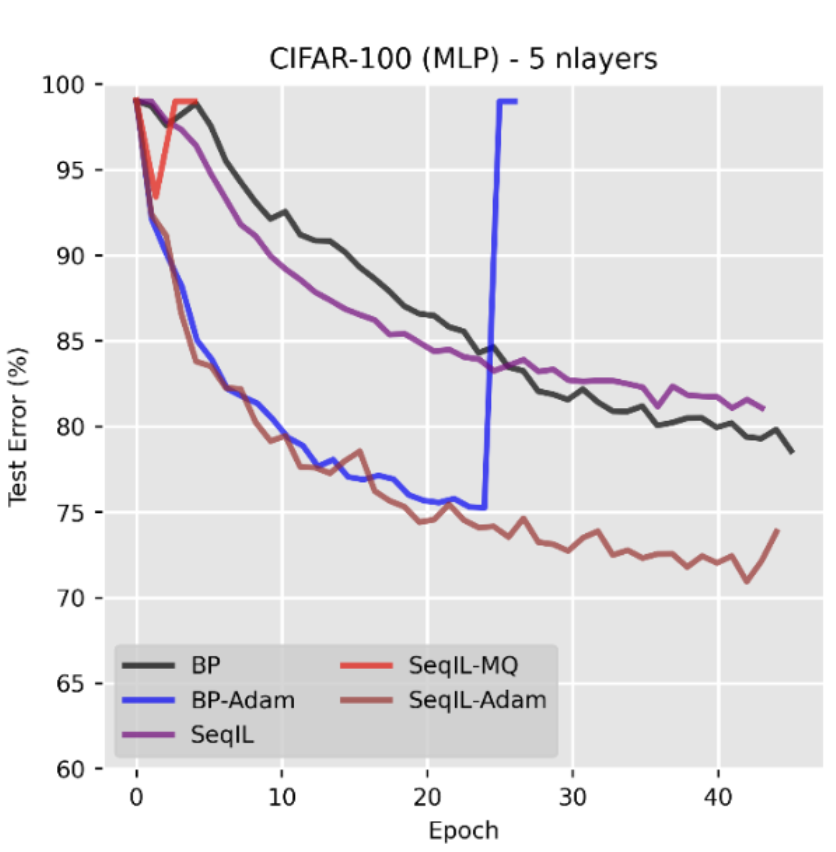
\includegraphics[width=\columnwidth, height = 0.3\paperheight]{images/cifar_mlp_1_5.png}}
\centerline{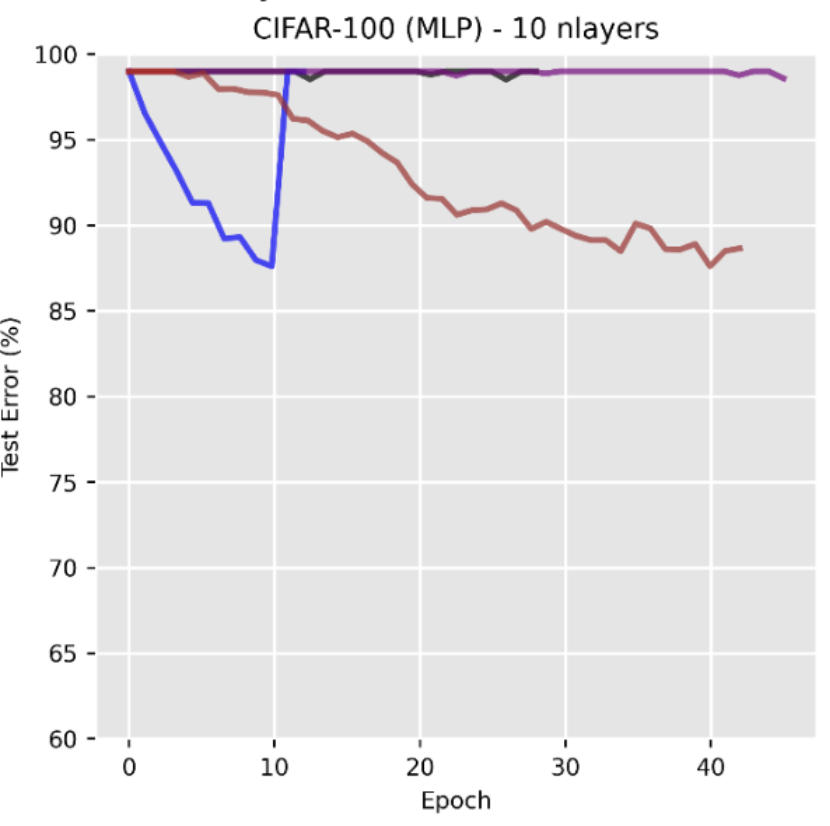
\includegraphics[width=\columnwidth, height = 0.3\paperheight]{images/cifar_mlp_1_10.png}}

\begin{figure*}[t]
    \centering
    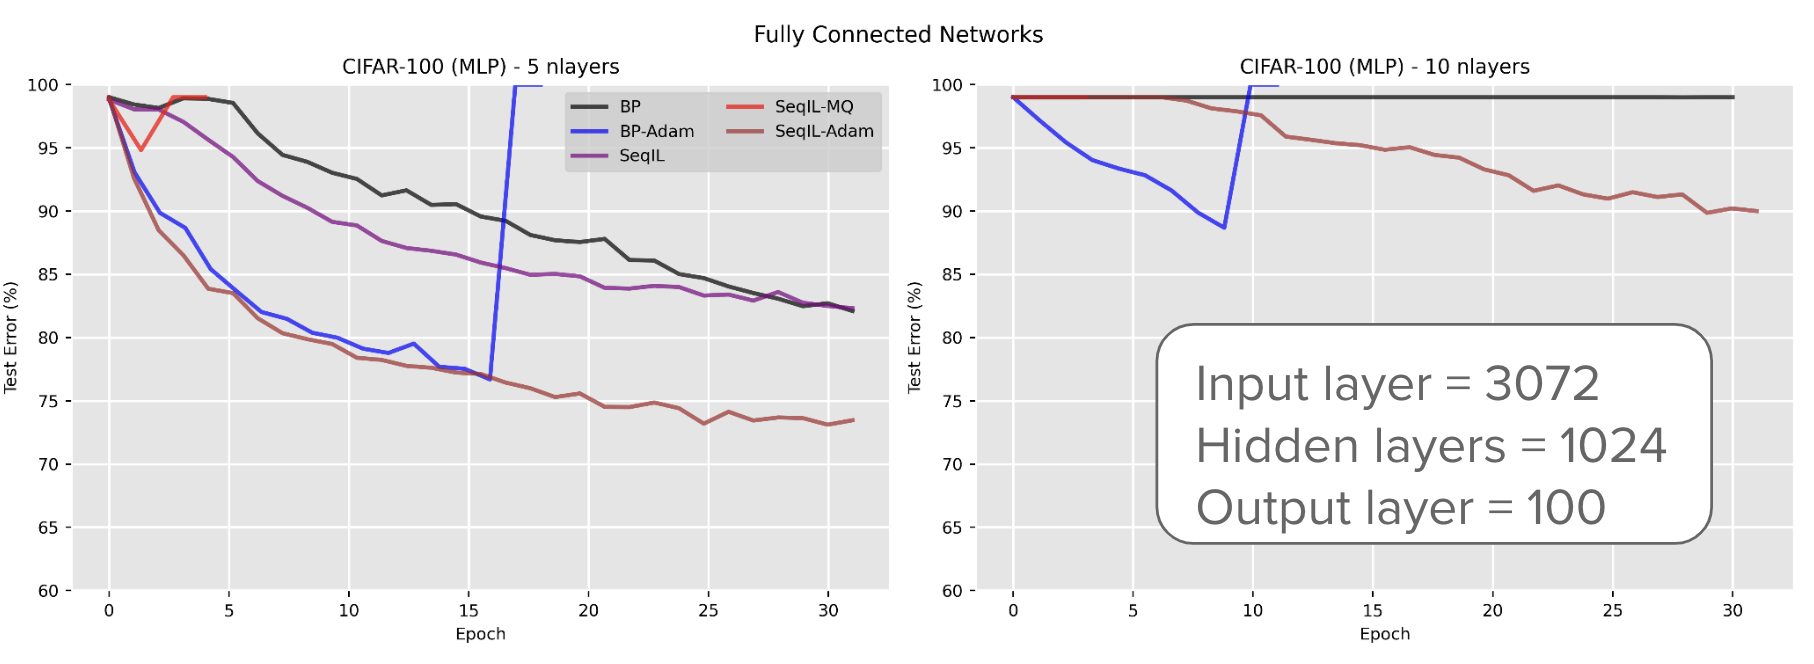
\includegraphics[width=\textwidth]{images/cifar_mlp_2.png} % Replace with your image file name
    \caption{CIFAR-100 MLP Run 2, with 5 and 10 hidden layers}
\end{figure*}

\begin{figure}[ht]
    \centering
    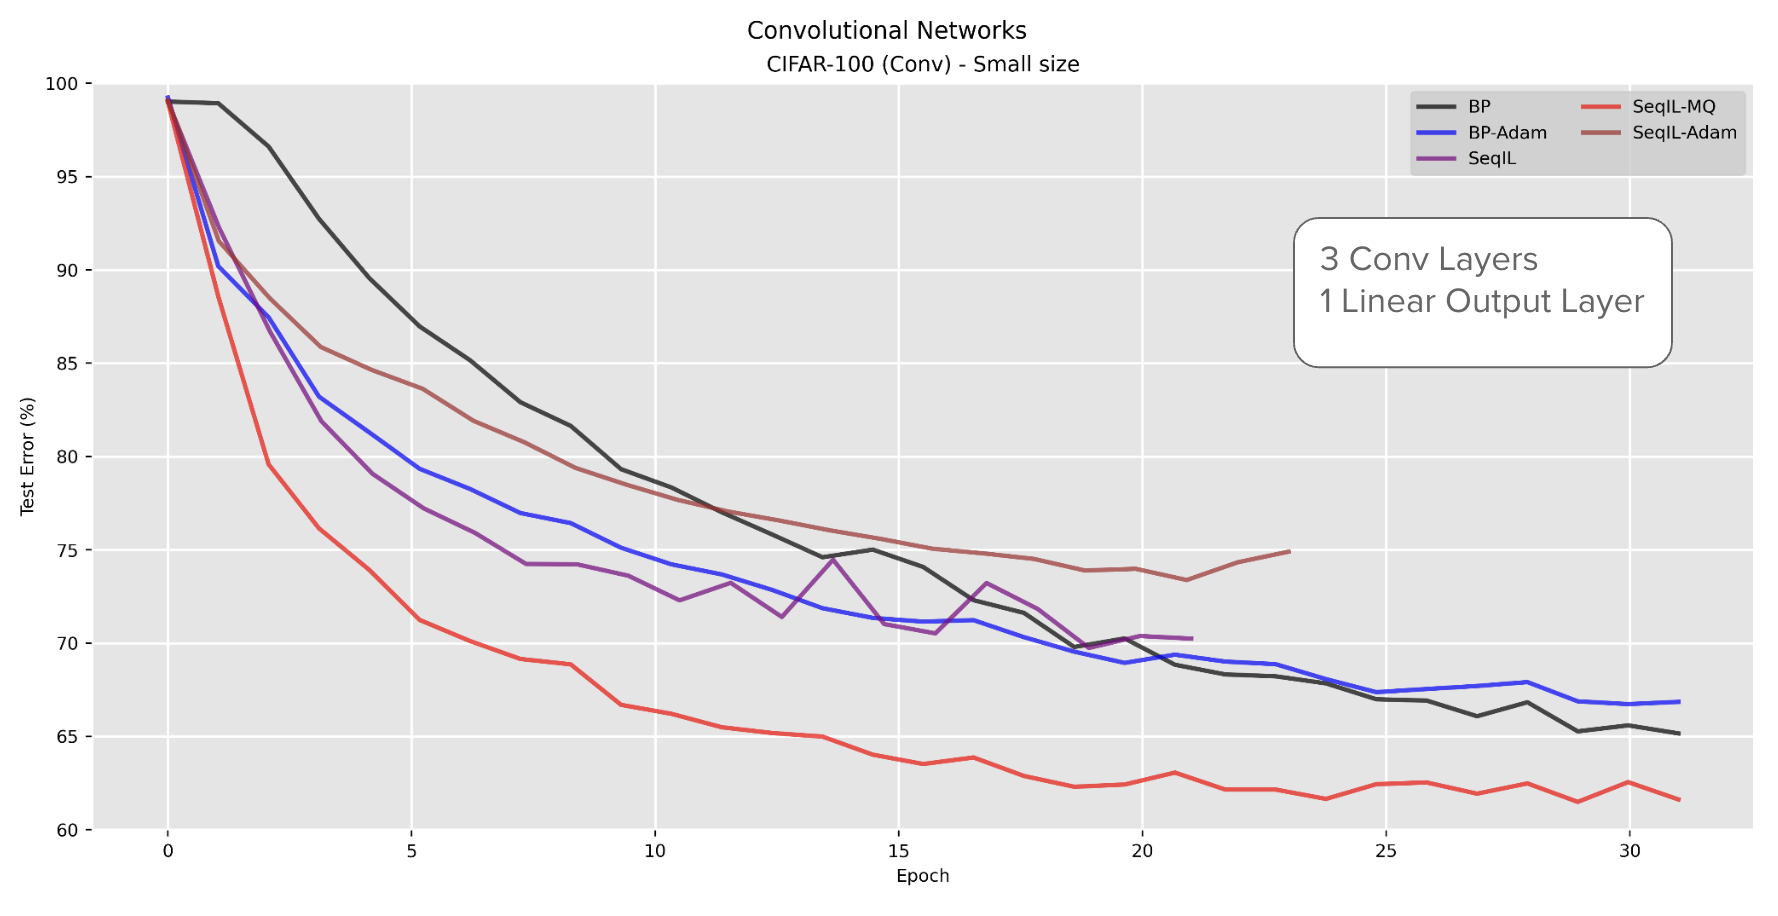
\includegraphics[width=\columnwidth]{images/cifar_conv_run1.png} % Replace with your image file name
    \caption{CIFAR-100 CNN Run 1, with batch size 64 and T = 3}
\end{figure}

Testing on MLP had the least promising results. From the above graphs of the 
first run on CIFAR-100 with 5 and 10 hidden layers we can see that while SeqIl-Adam performs the 
best with its performance being comparable to BP-Adam, SeqIL-MQ is nowehere to be seen. From the results,
it seems this model was unable to really learn anything and was not even able to reduce its error from 100\%.
It is strange to see BP-Adam perform well only to spontaneously lose all its learning and return to 
100\% error rate without any future improvement. This happens in both 5 and 10 layers runs of the model, and 
happens again when I run the same model again to see whether this was simply a bad random seed. 

It is notable that on the 10 layer network all algorithms perfomr significantly worse than on the 5 layer 
network. Here normal SeqIL and BP without any advanced optimizers fail to learn at all,
whereas their counterparts in the 5 layer network were still able to reduce error percentage by a decent amount of 
almost 20\%. For SeqIL this might be perhaps due to the truncated Inference Phase being too low for it to achieve 
adequate Free energy minimization thus leading it to be unable to learn at all, as well as the likely small updates that 
prevent it from updating its weights significantly. I ran this network many times after investigating the code for any bugs,
but was unable to discover why the BP-Adam algorithm undergoes an almost spontaneous collapse and was thus 
unable to remedy it either. 

Though SeqIL-Adam seems to be the most promising algorithm out of the bunch, we cannot ignore 
that this is still the least important variant as its memory costs are still very high. 

\subsection*{CNN}

\subsection*{CIFAR-100}

From Figure 4, we can see that while we there are a lot of issues not just for 
SeqIL-MQ in the MLP architecture, we have none in the CNN framework. We can see that standard 
BP in the end has comparable performance to BP-Adam but that BP-Adam is able to reduce 
Test Error much faster than regular BP. SeqIL-Adam surprisingly performs the worst of the bunch 
even comapred to Standard SeqIL and BP. SeqIL performs comparably to both BP and BP-Adam.
However, SeqIL-MQ performs the best by far out of the variants we observe. Not only does it achieve a better final 
test error rate after 30 epochs but it reduces it significantly faster than even BP-Adam.
This reinforces the ideas mentioned in the Alonso et al paper surrounding IL's sensitivity to second 
order information, which is exactly the kind of information Adam incorporates to make better gradient updates and thus 
reduce loss/error faster. Note that this is still in the case of a small model with 3 Convolutional layers.

\begin{figure*}[ht]
    % \vskip 0.2in
    \begin{center}
        \centerline{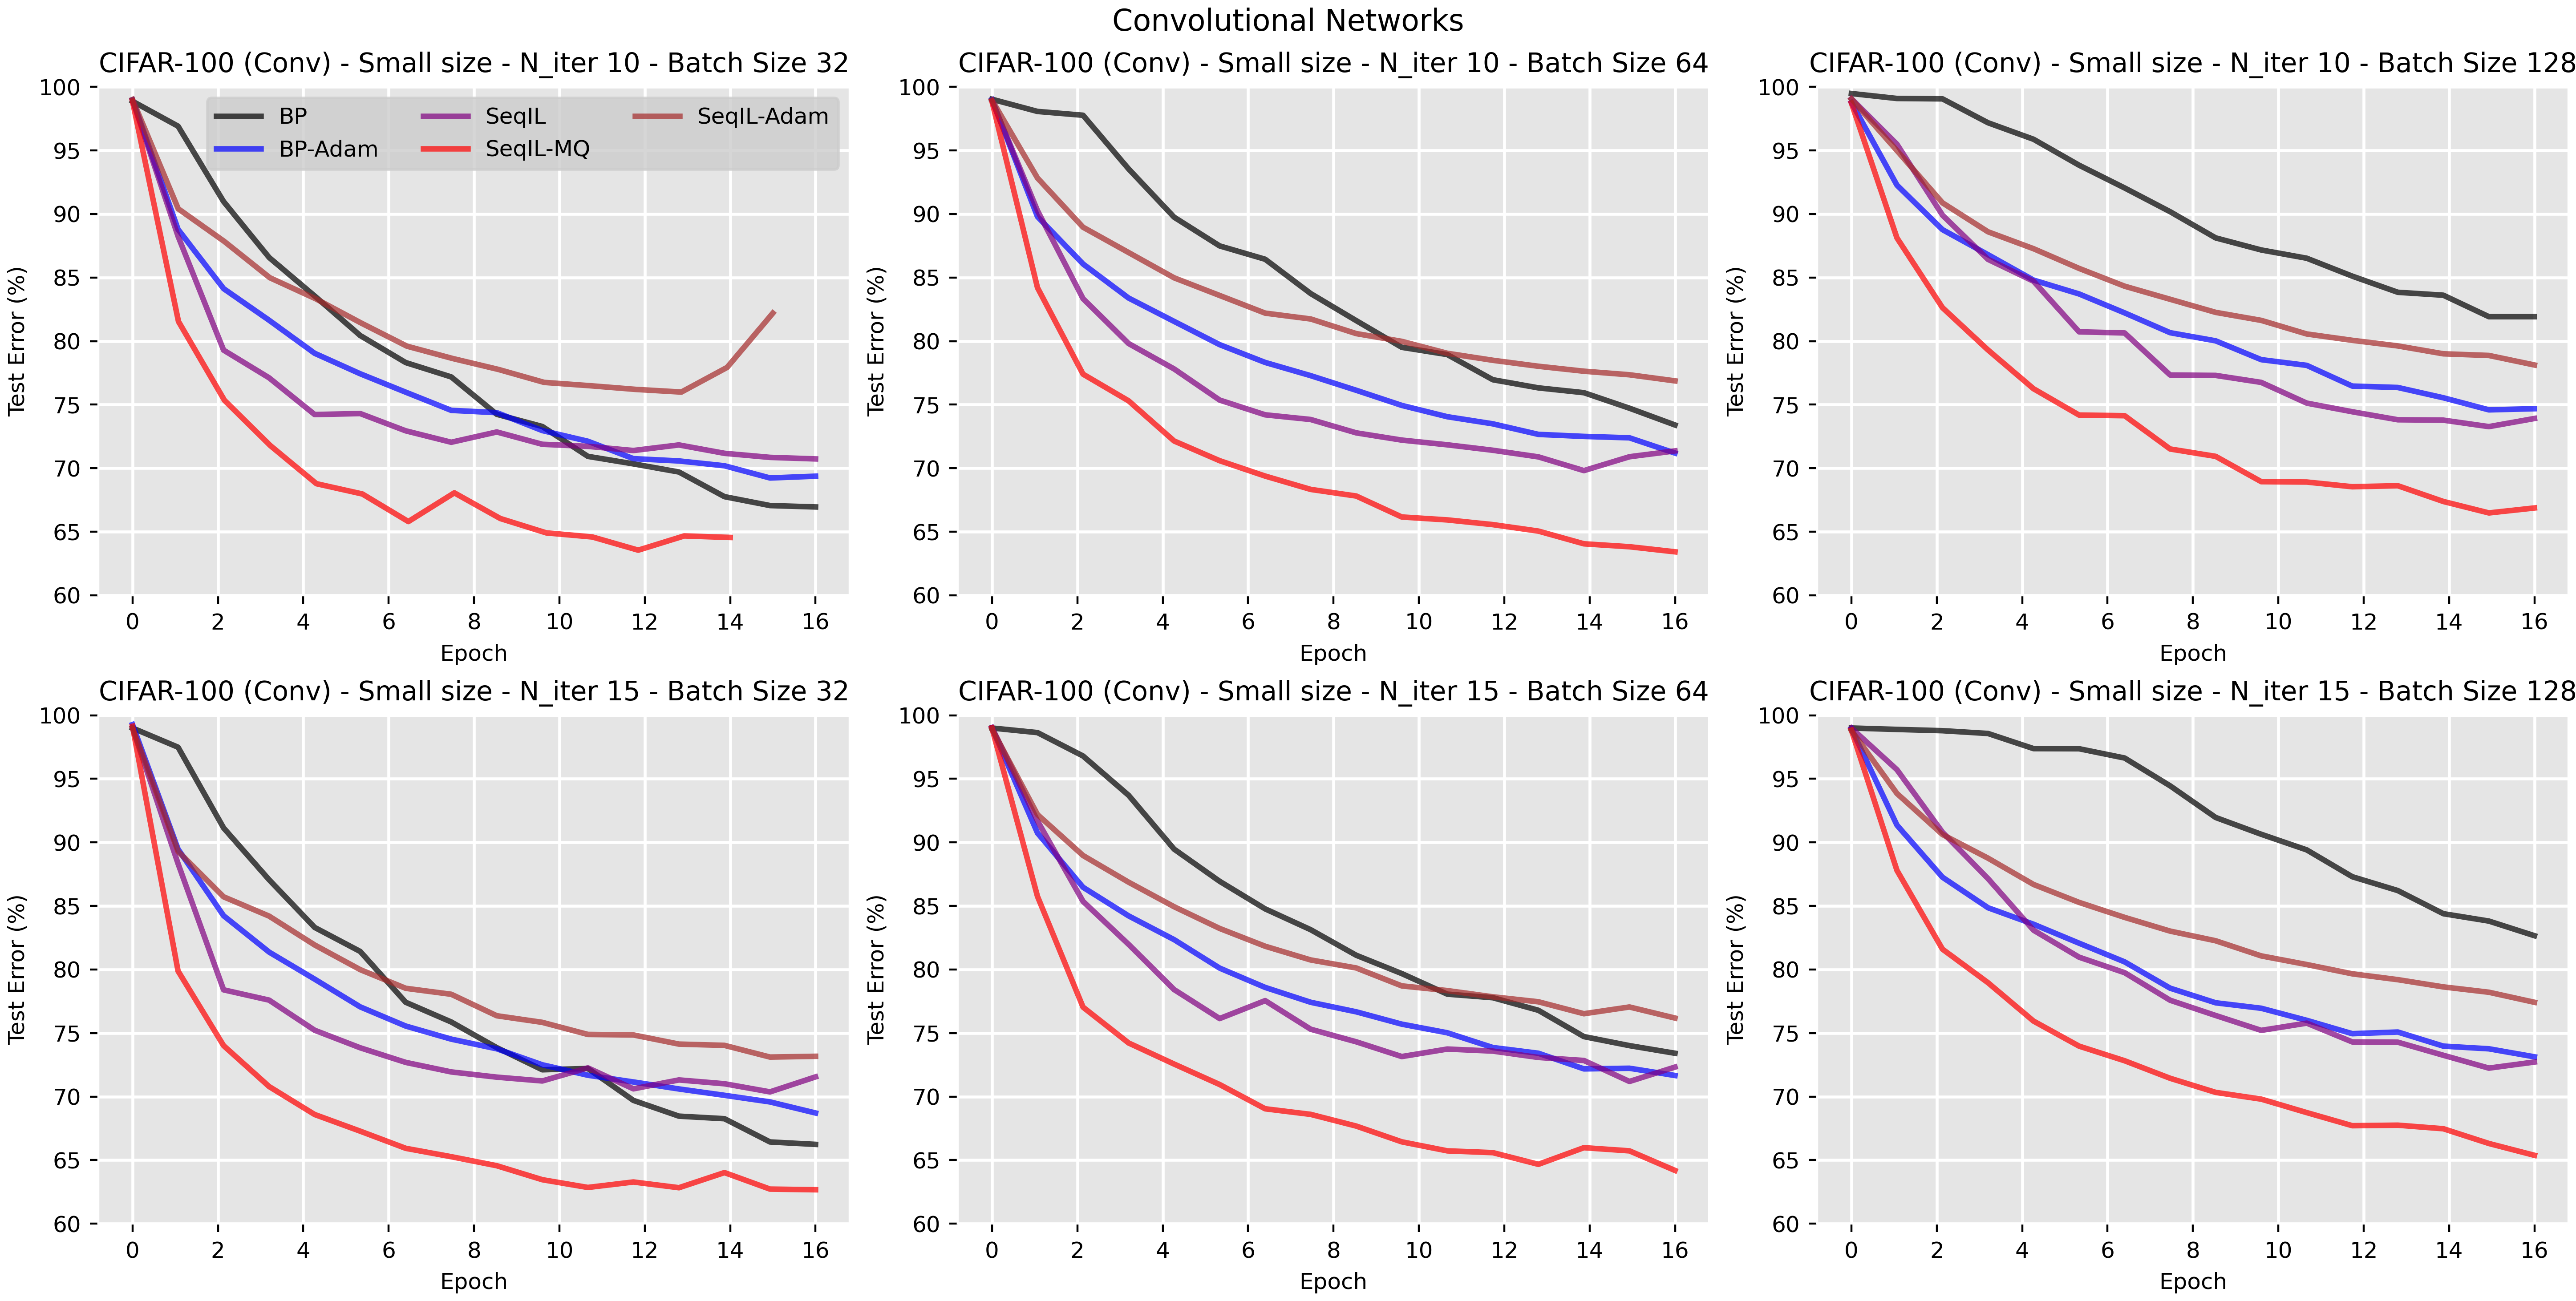
\includegraphics[width=\paperwidth]{images/cifar_run3_results_alt.png}}
    \caption{CIFAR-100 CNN with batch sizes = [32,62,128] and T=[10,15]}
    \end{center}
    % \vskip -0.2in
\end{figure*}

In Figure 5, I compare the performance of the CNN network for these various algorithms when using 
Inference phase iterations of 10 and 15 as well as batch sizes of 32, 64, and 128. This figure shows 
how different cobinations of iteration count and batch size affect the test error over 15 epochs which the 
models were run for. This was done because Alonso et al mentioned in their paper that they wished to test their models 
with different batch sizes and the different iteration counts was done to see if running it for longer 
would have some significant impact on the final error rate. Though they produced results 
suggesting that the truncated Inference phase was sufficient, I wanted to see if that would translate over into classification 
tasks that had more output classes. 

From these graphs we can tell that SeqIL-MQ perfomed the best for all combinations of these hyperparameters.
It is the algorithm that reduces error most quickly and achieves the lowest final error rate. There is no
significant difference between the final test errors amongst all the different hyper parameter combinations for SeqIL-Adam
however the rate of reduction looks to increase with smaller batch sizes. There may yet be an effect from 
the inference phase iterations but it is not noticeable from these results. Future testing is likely required.

It is also interesting how SeqIL-Adam seems to consistently perform the worst in terms of 
final test error rate on all these variations. BP, BP-Adam, SeqIL seem to have similar performance in both rate of 
error reduction and final test error rate.

It is also interesting to note that the test error seems to flatten out around 15 epochs suggesting 
perhaps only incremental improvements in model accuracy after this. However, the accuracy is at 40\% with 
the test error rate being 60\%. Perhaps this suggests that larger model sizes are required to capture 
the information and underlying patterns of this dataset with 100 classes. More testing should be done with larger 
model sizes to see if significantly better model accuracies can be achieved.

\subsection*{LabelMe50K}

\centerline{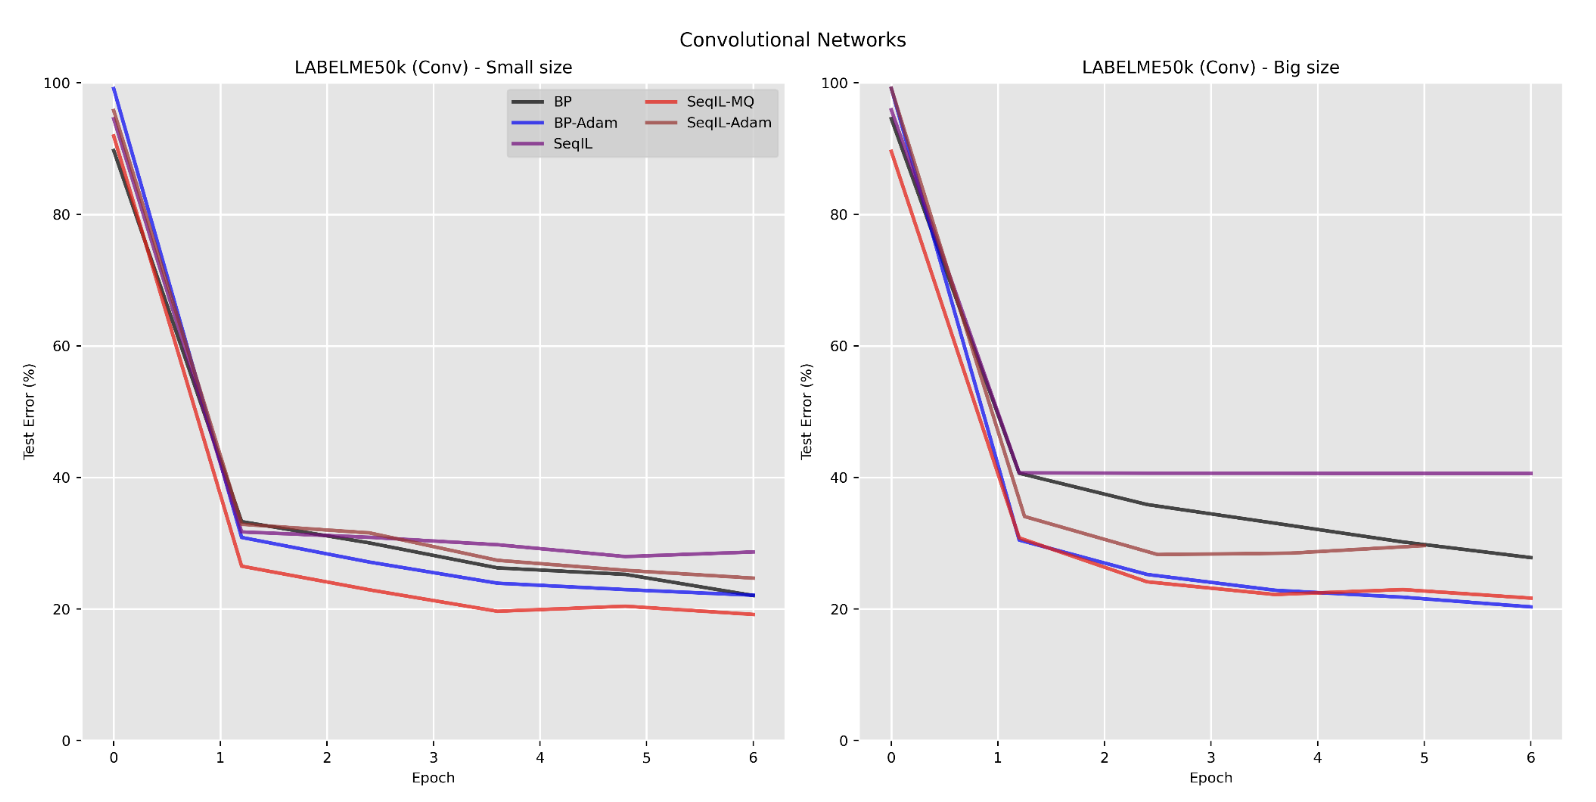
\includegraphics[width=\columnwidth]{images/LabelMe.png}}

\begin{figure*}[ht]
    % \vskip 0.2in
    \begin{center}
        \centerline{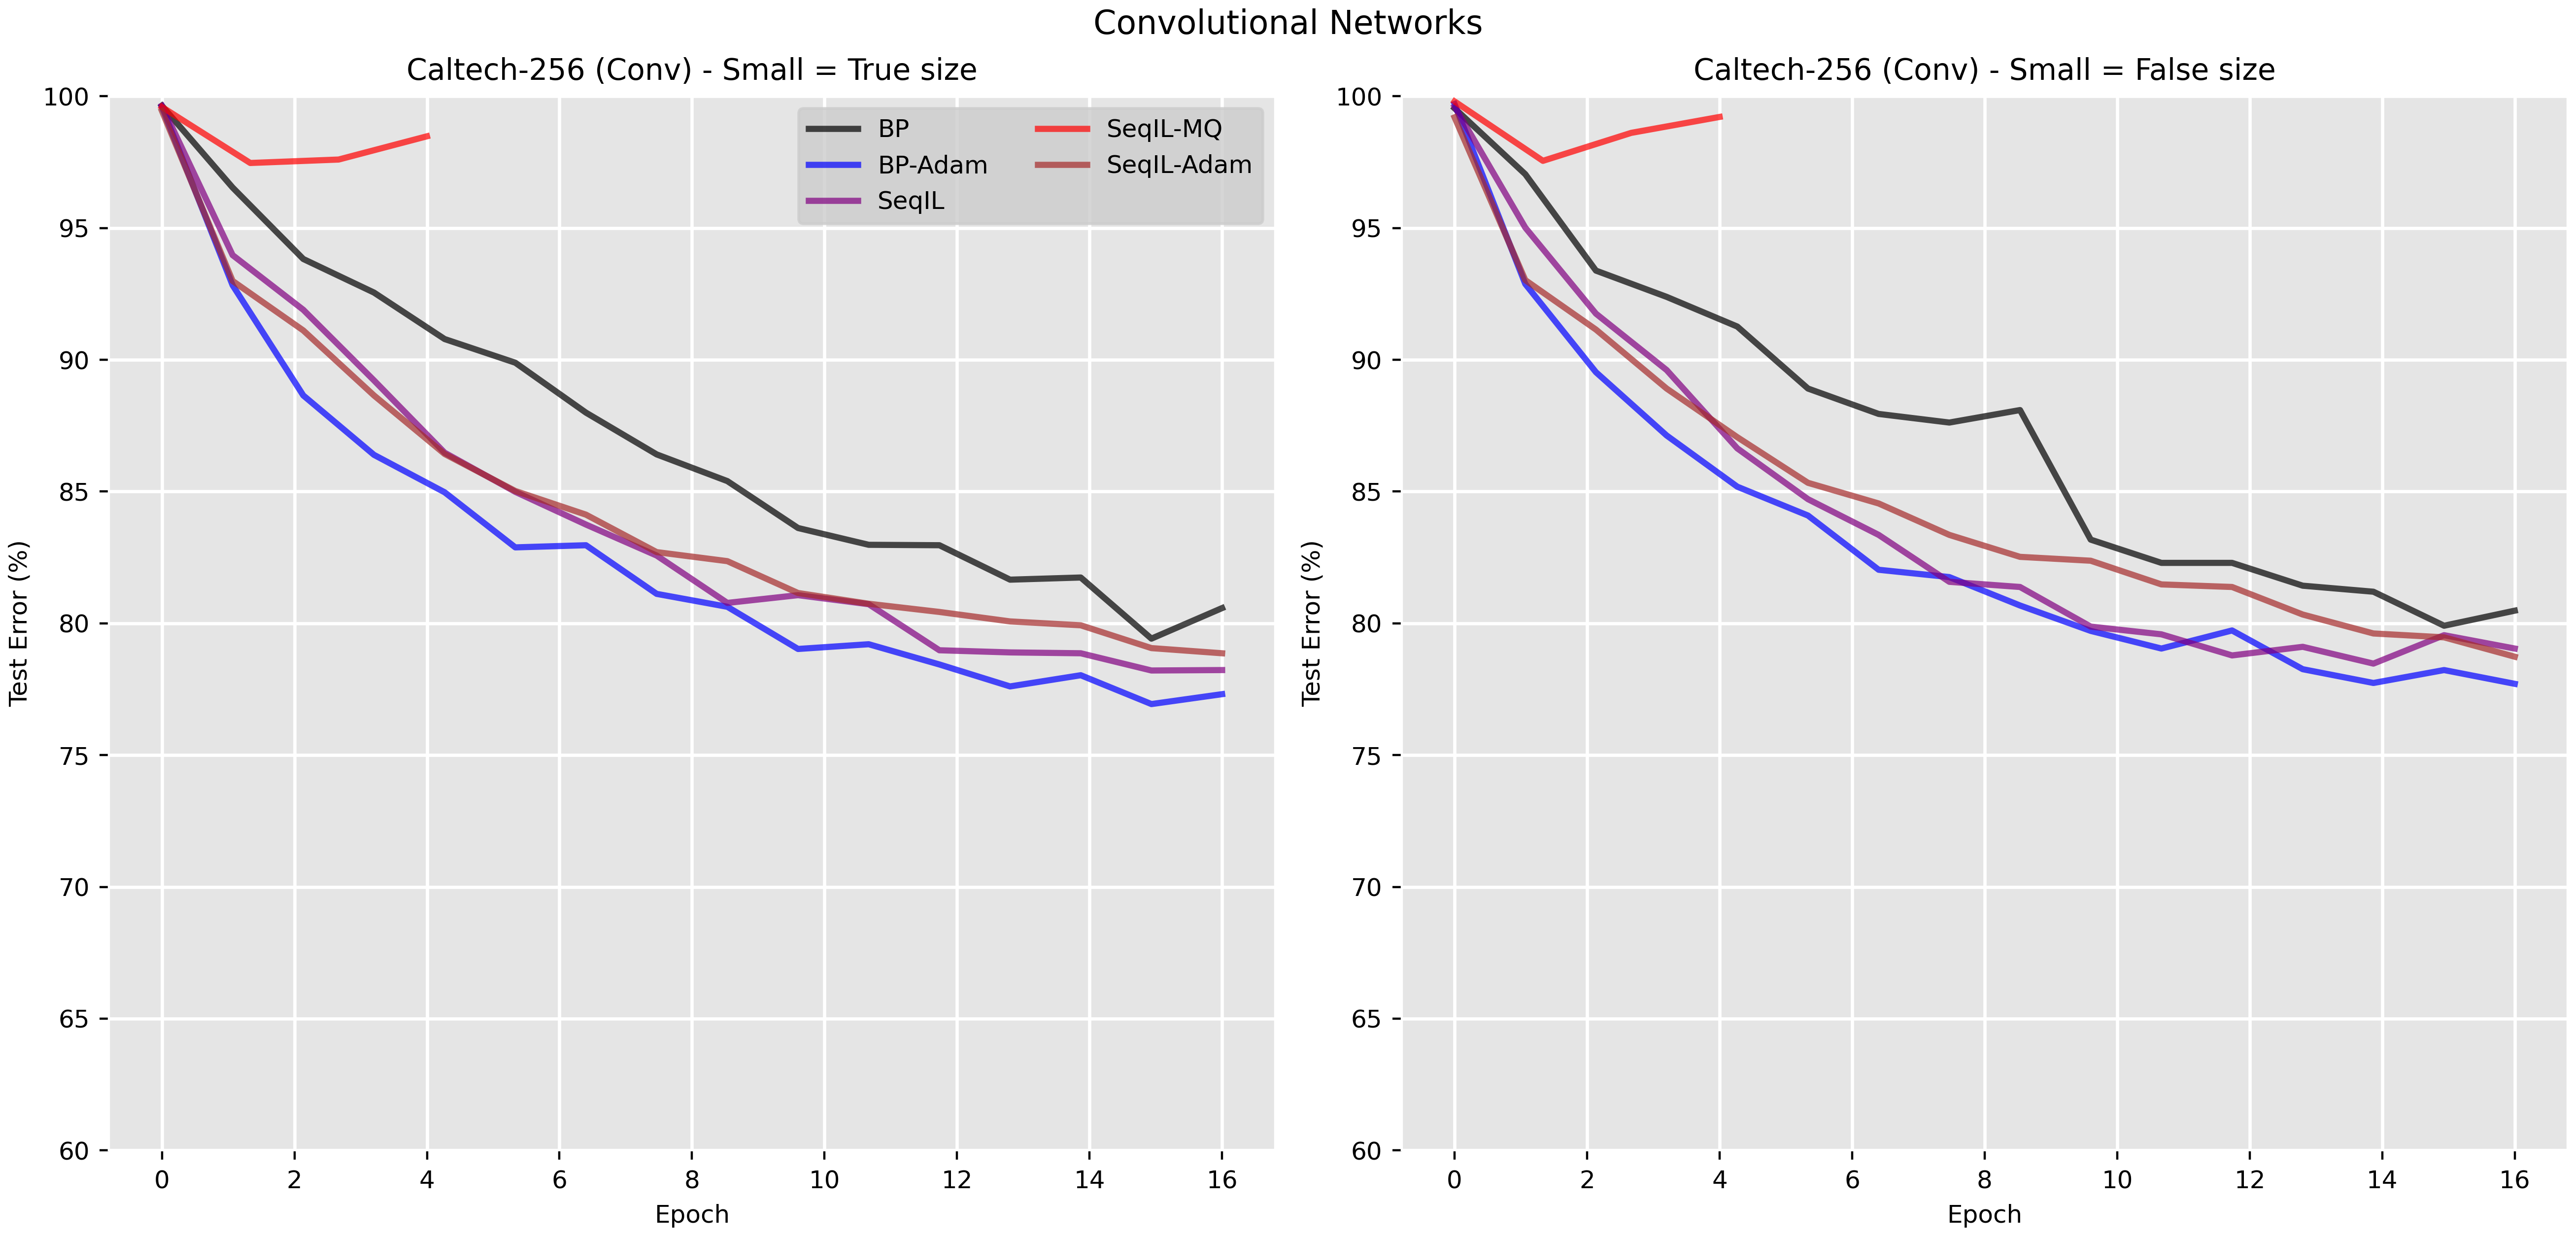
\includegraphics[width=\paperwidth]{images/caltech-256_results.png}}
    \caption{Simulataneous Inference vs Sequential Inference}
    \end{center}
    % \vskip -0.2in
\end{figure*}

The LabelMe50K results are not as interesting. All models perform similarly with SeqIL-MQ
still performing the best though the improvements are likely not significant. It still manages 
to reduce the test error faster and achieve a lower final test error rate across both model sizes.
It is interesting how the models without optimizers and again SeqIL-Adam perform significantly worse on the larger
model, which is important to remember that this model only has 2 more convolutional layers than its small
counterpart. More testing should be done to see if this difference and deterioration is exaggerated 
by even larger model sizes.

\subsection*{Caltech-256}

The Caltech-256 results are the most interesting. They show the first case of the 
breakdown of the SeqIl-MQ algorithm in the CNN architecture. So far it has performed well
on both the CIFAR-100 and LabelMe50K datasets showing significant learning and often the optimal performance 
of the models we are comparing it against. However here, the model seems to almost 
collapse after the first few epochs, failing to recover and never ending up with a
test error rate below 100\%. However SeqIl and SeqIl-Adam which has notoriously been the worst 
performing model across the previous datasets have comparable perfomrance with both BP and BP-Adam. 
Both SeqIl variants have comparable speed in test error reduction like BP-Adam and end up 
with final test error rates that are not significantly different from those of BP-Adam.

However, the test error rate is still around 77\% after 15 epochs and showing signs of 
flattening out and likely more epochs will only show incremental improvements thus suggesting
the model architecture is not complex enough to truly learn the underlying patterns for the 
257 categories represented in the dataset. 

\section{Conclusion}

In conclusion, more investigative work is needed for all models' performance on MLP models as there 
were a lot of anomalous results that require explanation of refutal. The CNN models however had great performances
by all models and highlighted how performant SeqIL-MQ really is. 

Similarly it seems we can conclude that lower batch sizes improve the rate of test error reduction but not the overall
accuracy significantly. Likely the Iteration count in the inference phase has negligible effect on 
model performance. 

In the case of Caltech-256 we can see that the MQ optimizer might work well for small datasets with 
small output classes, but as the model scales perhaps the MQ optimizer is unable to keep up. We can see this 
as where the Adam optimizer and base SeqIL were able to perform comparably to
BP-Adam, SeqIL-MQ was not. This suggests there is something about the weight updates that work
on a small scale that doesn't translate as the complexity of the dataset we are trying to model increases.

The accuracy rates for the various models we tested on showed learning but for CIFAR-100 the best we were able to get is 
40\% accuracy while for LabelMe we were able to get 80\% accuracy. For Caltech-256 we were only able to get 25\% accuracy.
This suggests that at least the smaller CNN models we were able to use perform better with fewer output classes to model.
Perhaps larger models will be able to increase our accuracies for both CIFAR-100 and Caltech-256.

\section{Future Work}

I was only able to implement model sizes of 3 and 5 convolutional layets respectively. It is imperative to test models
of even larger sizes such as 10 and 20 hidden layers to properly gauge how these optimizations and changes to base IL 
improve its performance and viability. I was limited by my compute and time budget and thus was unable to properly investigate 
larger datasets like SUN397 and use larger models with 10-15 hidden layers as I intended to do. 
Real time comparisons of these various algorithms on different model architectures will be useful to guide 
feasibility of its use in large scale models and guide what improvements still need to be had before it can be 
adopted en masse. 

More research needs to be done into alternative optimizers like MQ and tested against more complex datasets such as Caltech-256
to determine their efficacies. 

\section*{Code}

The repository for code modifications I made to the fork of the repository by Alonso et al can be found \href{https://github.com/rmohnani/PredictiveCoding-MQSeqIL}{here}.

% In the unusual situation where you want a paper to appear in the
% references without citing it in the main text, use \nocite
\nocite{langley00}

\bibliography{example_paper}
\bibliographystyle{icml2024}


\end{document}


% This document was modified from the file originally made available by
% Pat Langley and Andrea Danyluk for ICML-2K. This version was created
% by Iain Murray in 2018, and modified by Alexandre Bouchard in
% 2019 and 2021 and by Csaba Szepesvari, Gang Niu and Sivan Sabato in 2022.
% Modified again in 2023 and 2024 by Sivan Sabato and Jonathan Scarlett.
% Previous contributors include Dan Roy, Lise Getoor and Tobias
% Scheffer, which was slightly modified from the 2010 version by
% Thorsten Joachims & Johannes Fuernkranz, slightly modified from the
% 2009 version by Kiri Wagstaff and Sam Roweis's 2008 version, which is
% slightly modified from Prasad Tadepalli's 2007 version which is a
% lightly changed version of the previous year's version by Andrew
% Moore, which was in turn edited from those of Kristian Kersting and
% Codrina Lauth. Alex Smola contributed to the algorithmic style files.
